\section{Entwicklung einer Cross-kompilierten Applikation mit Flutter}
Der dritte Ansatz ist eine Cross-kompilierte Implementierung mit Hilfe des Flutter Frameworks.

\subsection{Flutter Grundlagen}
Flutter ist ein 2017 von Google veröffentlichtes Framework das mittlerweile zum meistgenutzten Cross-Plattform-Framework geworden ist \cite{statist_CP_Framework}. Die Aufmerksamkeit um Flutter lässt sich auch darin sehen, dass etwa Canonical\footnote{https://canonical.com/} , die Firma hinter Ubuntu, angekündigt hat, dass alle von ihnen entwickelten Anwendungen, in Flutter programmiert werden\cite{Ubuntu_Flutter}. Als Programmiersprache wird dabei Dart benutzt, die je nach Plattform, mit einem Compilern in nativen Code übersetzt wird.

Eine Grundlage von Flutter ist, dass alles auf dem Bidlschirm angezeigte ein Widget ist. Neben den tatsächlich angezeigten Elementen der Oberfläche können auch Gestenerkennung, Layouthelfer oder Logik durch ein Widget eingebunden werden \cite{Thiele_2018}. Dabei werden Widgets baumartig verschachtelt, wobei die meisten Widgets wieder ein oder mehrere Kinderelemente der Klasse Widget besitzen können. In Abbildung \ref{fig:flutter_layout_tree} etwa ist der Widget-Baum einer Menüleiste zu sehen. Ein Container ist dabei ein Element, das andere Widgets enthälten und etwa einen Abstand zu anderen Elementen definiert. Er ist mit dem div-Element von HTML vergleichbar. Bei Widgets wie in diesem Fall etwa Text oder Icon, stoppt der Baum, da diese keine weiteren Kinder haben.

\begin{figure}[ht]
  \centering
  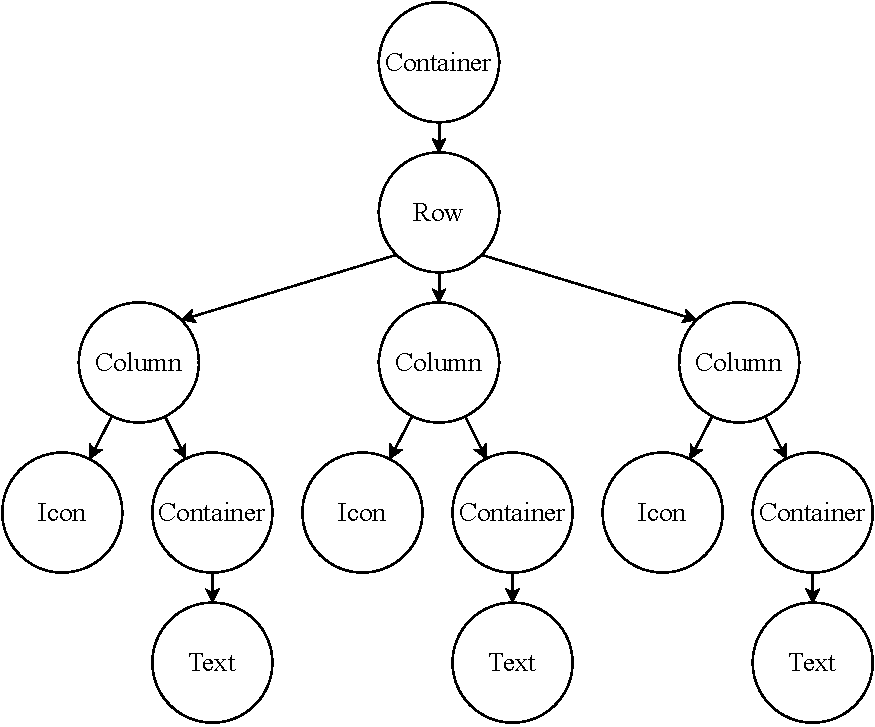
\includegraphics[height=8cm,keepaspectratio]{images/Flutter_menu_replacement.drawio.pdf} 
  \caption[Hierachie einer Menüleiste]{Hierachie einer Menüleiste\protect\footnotemark}
  \label{fig:flutter_layout_tree}
\end{figure}

\footnotetext{https://docs.flutter.dev/development/ui/layout}

Anders als bei der nativen Implementierung wird in Flutter das Layout mit der Funktionalität zusammen geschrieben. Das bedeutet, dass die Funktionalität direkt beim definieren eines Knopfes zugeordnet wird. Dafür muss lediglich das Widget in den Baum eingefügt werden und danach das entsprechende Attribut gesetzt werden. Dadurch ist alles an einem Ort.

Da Flutter einen großen wert auf Perfomance legt, ist eine Änderung auf der \ac{UI} so gebaut, dass nur Elemente neu gebaut werden, die ihren Inhalt geändert haben. Dafür hat Flutter für \verb|Stateful Widgets|, die eine extra State Klasse besitzen. In diesem werden Daten gespeichert und sobald er sich ändert, registriert Flutter die Änderung und baut daraufhin das geänderte Widget und die in der Hierachie folgenden neu\cite{9623025}. Dadurch kann häufiges und vor allem vollständiges Neubauen des Widgetsbaums verhindert werden. Jedoch benötigt nicht jedes Element einen State. Wenn etwa bereits zum Zeitpunkt des Erzeugens des Widgets, alle Daten feststehen und auch nicht mehr geändert werden, dann wird kein State benötigt und es reicht ein \verb|Stateless Widget| für die Implementierung\cite[Kapitel~4]{Flutter_Recipes}. Dadurch wird einerseits die Implementierung eines States ersparrt und bei einem Neubau des Baums, kann das Widget-Element wieder genutzt werden und muss lediglich neu gerendert werden, was bei Flutter jedoch sehr performant ist.

Um sich wiederholenden Code zu sparen, kann in Flutter einfach ein eigene Widget geschrieben werden, dass im gesamten Projekt wie jedes andere Element auch, in den Widget-Tree eingefügt werden kann. Das Erstellen eines Widgets ist dabei der selbe Prozess wie das erstellen einer Seite. Es wird ein Knoten Element gewählt und dann mit anderen Elementen kombiniert, um die gewünschte Oberfläche zu erhalten. Außerdem muss entschieden werden, ob es ein Stateful oder Stateless Widget ist. Je nachdem muss noch ein zusätzlicher State implementiert werden.


\subsection{Benutzte Plugins}
Das erste Plugin dass zu erwähnen ist, ist \verb|graphql\_flutter|\footnote{https://pub.dev/packages/graphql\_flutter}. Es ist ein Packet, dass ähnlich zu dem bereits erwähnten Apollo GraphQL einen Client zur Kommunikation mit einer GraphQL Schnittstelle. Damit der Client in allen Pages und Widgets verfügbar ist, muss die Konfiguration als Wurzel der Applikation gesetzt werden. Danach kann entweder über ein Widget oder über eine programmierte Funktion Die verschiedenen GraphQL Funktionen ausgeführt werden. Es ist ein Open Source von einer Community geschriebenes Plugin. Dies ist auch in der Nutzung spürbar. So sind einige Funktionalitäten nicht so sehr ausgereift wie bei der Apollo Implementierung. So muss etwa auf die einzelnen Felder der Antwort mit der JSON Zugriff \verb|Antwort.data[\"Feldname\"]|. Die Gefahr ist dabei hoch, dass durch ein Tippfehler der Zugriff schief läuft. Durch die Entwicklung von einer Community ist es allerdings einfacher Hilfe zu bekommen. So wurde während der Entwicklung ein paar Fragen auf dem dafür eingerichteten Discord-Server eingestellt, die professionell innerhalb einiger Stunden beantwortet wurden.

Das zweite wichtige Plugin ist Hive\footnote{https://pub.dev/packages/hive}. Es ist ein einfacher und schneller Key-Value Speicher, der Daten auhc über einen Neustart der App hinaus, in einer Datei innerhalb des Applikationsordner speichert. Er wird dafür genutzt, um den Identifikationsstring für den Server zu speichern. Es ist vergleichbar mit den \verb|SharedPreferences| der nativen Entwicklung vergleichbar, ist jedoch umfangreicher, da auch Objekte mit der richtigen Konfiguration gespeichert werden können und ist beim lesen vergleichbar beziehungsweise beim Schreiben schneller.

Ein drittes Plugin das hier noch erwähnt werden sollte ist \verb|simple_gradient_text|. Es ist ein Paket um ein Text mit Farbverlauf in der Schrift zu haben. Es ist also lediglich ein Paket, das zur Erstellung der Oberfläche genutzt wurde und ist dementsprechend hier nicht so wichtig. Jedoch zeigt sich hier wieder der Vorteil an einer aktiven Community. Bei der Installieren des Paketes gab es anfänglich einige Probleme, da es auf Android funktionierte aber auf anderen Plattformen nicht. Nach einer Unterhaltung mit dem Entwickler über ein erstelltes Problem auf GitHub ergab sich, dass das Plugin eine höhere Minimalversion von Dart benötigte, als in meiner Konfiguration eingestellt. Dadurch konnte bei mir der Fehler einfach behoben werden. Daraufhin wurde die Dokumentation des Paketes sowohl auf GitHub und dem zentralen Plugin Verzeichnis aktualisiert und um die entdeckte Anforderung erweitert.

Als letzte wichtige Bibliothek, wurde \verb|sqflite_common_ffi|\footnote{https://pub.dev/packages/sqflite\_common\_ffi} für die Implementierung der Datenbank genutzt. Es ist eine Bibliothek, dass auf Basis von \verb|sqlite3| eine Datenbankimplementierung für alle Plattformen anbietet.
Diese wird beim Start der Anwendung geöffnet und ist danach in der kompletten Anwendung verfügbar.
 Mit ihre können alle gängigen \ac{CRUD}-Operationen durchgeführt werden. Die Implementierung ist dabei denkbar einfach.
Zum erstellen der Tabelle muss lediglich der SQL Befehl zum erstellen ausgeführt werden und danach kann über dedizierte \verb|insert| und \verb|query| Methoden die Daten gespeichert beziehungsweise abgefragt werden.
Nebenbei kann jede Art von SQL-Befehl ausgeführt werden, um Befehle auszuführen, die über die normale Implementierung hinaus gehen.


\subsection{Exkurs: Platform spezifische Funktionalität entwickeln}
Im Verlaufe der Entwicklung kann es vorkommen, dass eine gewisse Funktionalität, die essentiell für die Anwendung ist, bisher nicht implementiert wurde oder die verfügbaren Bibliotheken nicht die gewünschte Funktionalität haben oder benötigte Plattformen nicht unterstützt werden. Für diesen Fall kann ein eigenes Plugin geschrieben werden. Der Aufbau eines solchen Plugins kann in Abbildung \ref{fig:flutter_plattform_specific} gesehen werden. Dabei wird einerseits der Dart-Code benötigt, der das Plugin definiert und die Daten eventuell weiterverarbeitet. Auf der anderen Seite steht der jeweilig notwendige Plattformcode, in dem die native Funktionalität implementiert ist. Zur Kommunikation ist dazwischen der sogenannte Plattform-Channel, der eine Kommunikation in beide Richtungen ermöglicht \cite[Kapitel~12.3]{Flutter_Recipes}.

\begin{figure}[ht]
  \centering
  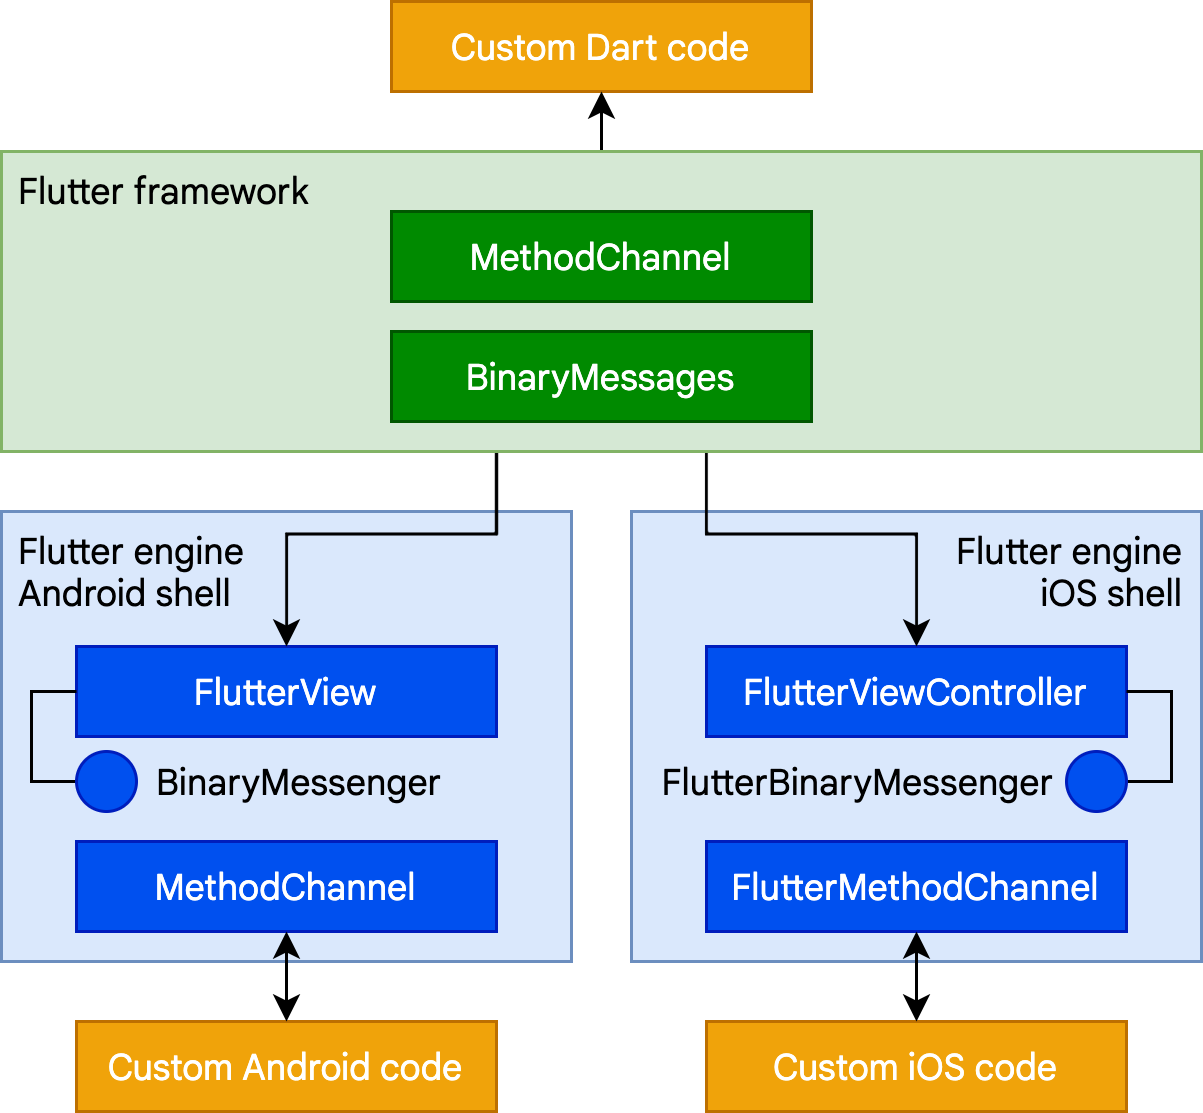
\includegraphics[width=9cm,keepaspectratio]{images/flutter-platform-channels.png} 
  \caption[Aufbau eines Plugins mit plattformspezifischen Code]{Aufbau eines Plugins mit plattformspezifischen Code\protect\footnotemark}
  \label{fig:flutter_plattform_specific}
\end{figure}

\footnotetext{https://docs.flutter.dev/resources/architectural-overview}

Durch die Nutzung dieser Kanäle wird gleichzeitig die Ausführung des Plattform Codes auf einem separaten Threads ermöglicht. Dadurch kann dieser asynchron ausgeführt werden und der Thread, auf dem die \ac{UI} ausgeführt wird, wird nicht blockiert\cite{plattform_code_flutter}.

Es ist also möglich benötigte Funktionalität hinzuzufügen, solange sie auf den einzelnen Plattformen möglich ist. Jedoch wird hierfür der Code in der jeweiligen Programmiersprache der Plattform benötigt, was eine gewisse Kenntniss auf den Plattformen voraussetzt.

\subsection{Exkurs: Firebase}
Ein weiterer Aspekt, warum Flutter gerade bei kleineren App-Projekten gern genutzt wird, ist die umfangreiche Integrationsmöglichkeit von Firebase. Eine aktuelle Untersuchung ergab, dass in Android Applikationen die eine Analyse Software integriert haben, 92\% der weltweiten Applikationen, Firebase nutzt \cite{statist_analytics_SDK}.

Firebase ist eine Backend-as-a-service Lösung, die dabei helfen soll, schnell und einfach Anwendungen zu entwickeln und zu betreiben\footnote{https://firebase.google.com/}. Es ist also eine Sammlung von verschiedensten Tools und Plugins, die einem Entwickler die Möglichkeit geben soll, sich auf Design und Funktionalität der App konzentrieren zu können. Es umfasst Tools wie eben Analyse Software um Nutzungsdaten zu sammeln und zu analysieren, ein fertiges Chatsystem oder auch eine Cloud gestützte Datenbank Lösung. So schreiben Guzzi et Al, dass entweder ein Team an Entwickler angestellt werden müssten, das in monatelanger Arbeit ein Backend System programmieren würde, um dann eine Schnittstelle zu einem Backend zu bauen. Andererseits kann auch ein bereits bestehendes System gennommen werden. Mit Firebase werden tausende Zeilen Code eingespart und erhält dabei die Möglichkeit, asynchrone Aufrufe und nebenläufige Prozesse für eine reaktive App zu nutzen \cite[p.~608]{Flutter_Apprentice}.

Um eine Datenbank für seine App zu erstellen sind es wenige Schritte. So kann auf der Webseite von Firebase eine neue Datenbank angelegt werden. Danach wird die erzeugte Konfigurationsdateien für die jeweiligen Plattformen heruntergeladen. Diese werden den jeweiligen Implementierungen hinzugefügt. Danach müssen die Datenstrukturen lokal in der App entworfen werden und eine Verbindung hergestellt. Dafür werden die Daten-klasse mit JSON Konvertierungen, ein \ac{DAO} mit einer Methode zum speichern und holen der Daten und zuletzt noch einen Provider erzeugt. Außerdem besteht die Möglichkeit, neben einer online Datenbank ebenfalls eine offline Version hinzuzufügen, die synchronisiert wird, sobald eine Internetverbindung hergestellt wird \cite{Flutter_Apprentice}.

Ein weiterer Pluspunkt ist die Integration von Firebase-Authentifizierung. Es bietet eine fertige Lösung zur Authentifizierung von Nutzern. Es besteht außerdem die Möglichkeit, Benutzer zu kategorisieren beziehungsweise die Nutzung einzuschränken. So kann über Regeln in der Firebase-Website, präzise definiert werden, welcher Nutzer auf welche Daten zugreifen kann. Weiter können Nutzer auch von der Nutzung des Dienstes ausgeschlossen werden oder nur bestimmte Emailadressen zugelassen. Es bietet also ein vielseitig und umfangreiches Nutzerverwaltungstool \cite{Flutter_Apprentice}.

Firebase ist natürlich nicht nur für Flutter verfügbar, sondern genauso für die verschiedensten Programmiersprachen der Plattformen Android, iOS oder auch Web. Dennoch ist Flutter und Firebase ein interessantes Gesamtsystem. Denn durch Flutter muss lediglich einmal der Code zum Zugriff auf die Datenbak oder die anderen Dienste geschrieben werden. So wird nicht nur weiter Entwicklungszeit um sehr ähnlichen Code zu schreiben, sondern verhindert gleichzeitig eine unterschiedliche Definition der Entitäten oder anderen Elementen. Außerdem ist dadurch ein problemloser Wechsel von einem System zu einem anderen Möglich, da alle Anwendungen auf egal welcher Plattform gleich sind.

\subsection{Fazit Flutter}
Durch die hier beschriebene Entwicklung kann mit Hilfe von einem Code, eine Anwendung geschrieben werden, die sowohl auf Android, iOS, Windows, Mac und Linux läuft. Lediglich die Web Implementierung funktioniert nicht, da der GraphQL Client hier keine richtige Verbindung erstellen kann. Für alle anderen Plattformen muss lediglich die Unterstützung deklariert, der Code in Plattform spezifischen Code compiliert und am Ende ausgeführt werden.

Das Tempo mit dem eine Flutter Anwendung entwickelt werden kann ist ähnlich wie eine einzelne native Implementierung. Dabei entsteht aber, wie bereits erwähnt, nicht nur die Implementierung für eine Plattform, sondern 5. Selbst wenn der Fokus der Entwicklung zuerst nur auf einer Plattform liegt, kann es sinnvoll sein Flutter zu nutzen um in Zukunft weitere Plattformen hinzuzufügen. Denn alle Plattformen können nachträglich noch exportiert werden.

Jedoch ist dies natürlich nicht immer möglich. Denn etwa der GraphQL Client ist nicht mit einer Web-Version kompatibel. Daher sollte bei der Wahl der Pakete darauf geachtet werden, welche Packete ausgewählt werden, um eine Inkompatibilität mit den gewünschten Plattformen zu verhindern. Wie bereits ausgeführt, kann versucht werden, solche Probleme durch eine eigene Implementierung zu lösen, dies ist jedoch mit einem erhöhten Aufwand und nötigen Wissen verbunden. Dabei ist die eigentliche Implementierung an sich nicht das eigentliche Problem, da auch hier dann native externe Bibliotheken genutzt werden können, jedoch ist die Konfiguration der Kommunikationsschnittstellen mitunter recht kompliziert und müssen sinnvoll implementiert sein, um die Performance nicht erheblich zu schwächen.

Flutter ist außerdem noch recht neu. So werden bei regelmäßigen Updates auch Änderungen eingeführt, die die Qualität und Entwicklung verbessern, jedoch dabei auch umfangreiche Änderungen in allen Applikationen notwendig macht. So wurde etwa ein Update veröffentlicht, dass das Nullsafety verbessern sollte. In Folge dessen musste jede Bibliothek angepasst und auch große Teile von Applikationen angepasst werden. Dadurch sind auch einige Anleitungen für Flutter veraltet und funktionieren in der aktuellsten Version nicht ohne Anpassungen.

Ein letzter Punkt ist, dass es keine Liste der verfügbaren Widgets innerhalb der Entwicklungsumgebung gibt. So muss alles, was nicht bereits bekannt ist gegoogelt werden. Hier wäre eine Übersicht über die typischen Elemente hilfreich um gerade für Anfänger den Einstieg zu erleichtern.